\chapter{Memory Management as a Service}
\label{chap:service}
The service layer, positioned above the OS layer, plays a pivotal role in facilitating efficient and seamless memory sharing across multiple computing and memory nodes within a disaggregated architecture. As application software, it provides greater flexibility than the operating system, allowing for a variety of services to be offered to applications. These adaptable services enable applications to choose options best suited to their specific needs. However, this requires that the storage and compute are easily decoupled, otherwise the application developers will need to spend enormous effort to modify the application for it to use memory management service. 

Serverless architecture offer on-demand elasticity of compute and storage and decouples them logically. Recent work on serverless analytics has demonstrated the benefit of using serverless architecture for resource- and cost-efficient data analytics. The key idea of serverless analytics is to use a remote low-latency, high-throughput shared far-memory system for (1) inter-task communication and (2) for multi-stage jobs, storing intermediate data beyond the lifetime of the task that produced the data. This makes it a perfect target for disaggregate memory since compute and memory are decoupled logically when the serverless task is assigned.

Designing a memory management service is a non-trivial tasks. Our discussion begins with an outline of the essential requirements for such memory management services, focusing on the unique challenges introduced by disaggregation. We then highlight our current efforts to tackle these challenges and explore potential directions for future research in this rapidly evolving domain.

\paragraphb{Elasticity}  Memory usage in modern computing environments can be highly variable, with applications experiencing fluctuating memory demands~\cite{jiffy}. Elasticity allows the memory service to dynamically allocate and deallocate memory resources based on current requirements, optimizing resource utilization. In typical applications with dynamic memory requirements, such as data analytics, applications are organized into jobs that contain multiple tasks. Each task can be assigned to run on an arbitrary compute node. Each task communicates with the other using memory as intermediate storage. Previous solutions ~\cite{pocket} tend to allocate resources in a job granularity. Jobs specify their memory demands before the job is submitted and the system reserves the amount of memory for the entire job lifetime. The tradeoff between performance and resource utilization for such job-level resource allocation is indeed well studied in prior work ~\cite{jiffy}. On the one hand, if jobs specify an average demand of memory, the job will degrade as running out of memory will lead to swapping data out to slower storage medium (e.g. S3 storage), while on the other hand allocating at peak granularity will result in resource wastage.

\paragraphb{Isolation} The second requirement is the isolation between different compute tasks. Since multiple computing threads can be using the same disaggregated memory pool, it's essential to multiplex between applications to improve resource efficiency but at the same time keep the memory of different threads isolated from each other, which means that the memory usage of a particular application should not affect other existing applications. The number of tasks reading and writing to the shared disaggregated memory can change rapidly in serverless analytics which makes the problem even more severe.

\paragraphb{Lifetime management}
Decoupling compute tasks from their intermediate storage means that the tasks can fail independent of the intermediate data, therefore we need mechanisms for explicity lifetime management of intermediate data.

\paragraphb{Data repartitioning}
Decoupling tasks from their intermediate data also means that data partitioning upon elastic scaling of memory capacity becomes challenging, especially for certain data types used in serverless analytics (e.g. key-value store). If it's the application's responsibility to perform such repartitioning, it will involve large network transfers betweem compute tasks and the far memory system and massive read/write operations every time the capacity is scaled. What's more, the application need to implement different partitioning strategies for different kind of data structures used. Therefore, new mechansims to efficiently enable data partitioning within the far memory system is essential.


We present Jiffy, an elastic disaggregated-memory system for stateful serverless analytics. Jiffy allocates memory resources at the granularity of small fixed-size memory blocks - multiple memory blocks store intermediate data for individual tasks within a job. Jiffy design is motivated by virtual memory design in operating systems that also does memory allocation to individual process at the granularity of fixed-size memory blocks(pages). Jiffy adapts this design to stateful serverless analytics. Performing resource allocation at the granularity of small memory blocks allows Jiffy to elastically scale memory resources allocated to individual jobs without a priori knowledge of intermediate data sizes and to meet the instantaneous job demands at seconds timescales. As a result, Jiffy can efficiently multiplex the available faster memory capacity across concurrently running jobs, thus minimizing the overheads of reads and writes to significantly slower secondary storage (e.g., S3 or disaggregated storage)

\section{Elastic memory management for data analytics}
\begin{comment}
\begin{figure}[t]
    \centering
    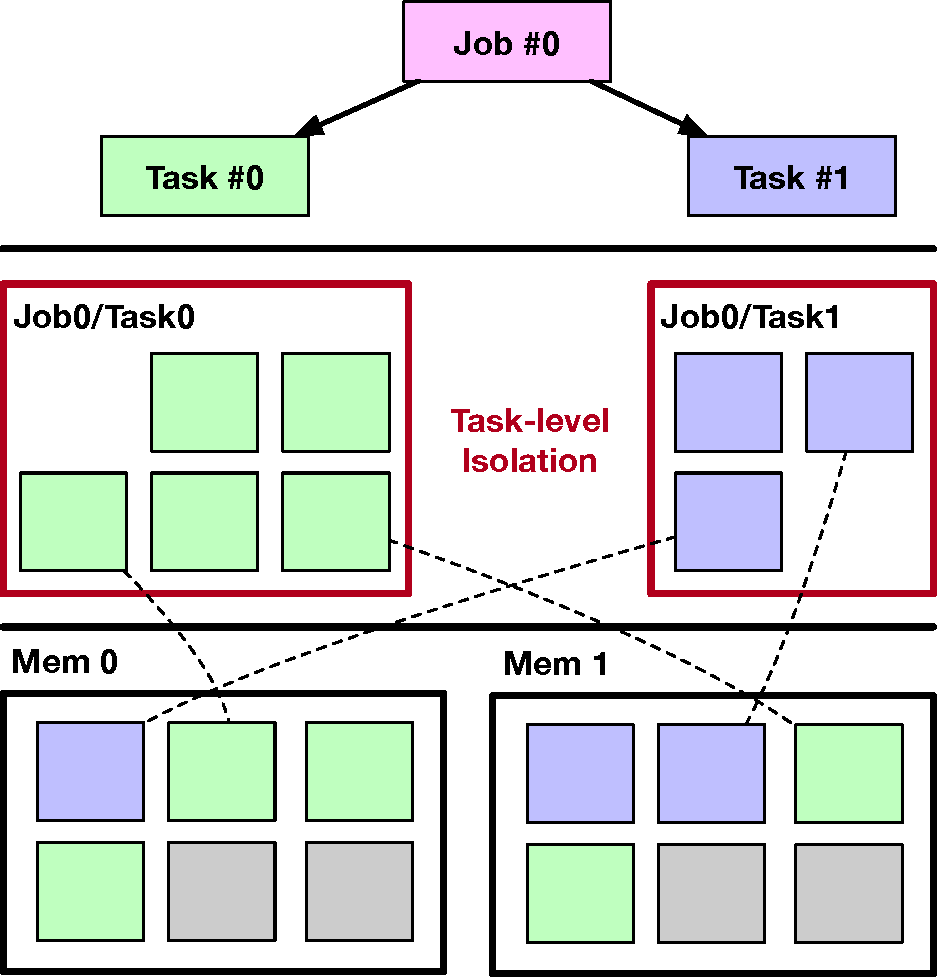
\includegraphics[width=0.6\columnwidth]{Jiffy.pdf}
    \caption{\textbf{Jiffy Overview.} Jiffy allocates memory resources individually for each task within a job. Memory is allocated in small, fixed-sized blocks to ensure elastic scaling of memory according to demand.} 
    \label{fig:jiffy} \vspace{-2.0em}
  \end{figure}
\end{comment}
Data analytics applications, which utilize disaggregated memory for inter-task communication and intermediate data storage, are becoming increasingly common. As discussed in ~\cite{starling, shuffling, pocket, cirrus}, these applications handle user requests in the form of jobs, each defining its memory needs upon creation. The dilemma of balancing performance with resource efficiency for job-level memory allocation has been extensively studied ~\cite{elasticquery, qoop}. If a job is based on average demand, performance may decline during peak demand periods due to inadequate memory, causing data spillage to slower secondary storage, such as SSDs. Conversely, allocating memory for peak demands leads to underutilization of resources when the actual demand is below peak. Evaluations on Snowflake's workload, as shown in ~\cite{elasticquery}, indicate a significant fluctuation in the ratio of peak to average demands, sometimes varying by two orders of magnitude within minutes.

In response to the challenges of dynamically allocating memory resources in data analytics applications, we have developed Jiffy~\cite{jiffy}, an elastic memory service tailored for disaggregated architectures. As shown in Figure \ref{fig:jiffy}, Jiffy allocates memory in small, fixed-size blocks, enabling the dynamic adjustment of memory allocation for individual jobs without prior knowledge of intermediate data sizes. Jiffy employs a hierarchical address space that reflects the structure of the analytics job, facilitating efficient management of the relationship between memory blocks and tasks while ensuring task-level isolation.

\section{Introduction}


Serverless architectures offer flexible compute and storage options, charging users for precise resource usage. Initially used for web microservices, IoT, and ETL tasks, recent advancements show their efficacy in data analytics. Serverless analytics leverage remote, high-throughput memory systems for inter-task communication and storing intermediate data. However, existing far-memory systems face limitations, allocating resources at the job level, leading to performance issues and underutilization.

To address this, we introduce Jiffy, an elastic far-memory system for stateful serverless analytics. Unlike conventional systems, Jiffy allocates memory in small, fixed-size blocks, enabling dynamic scaling and efficient resource utilization. This approach resolves challenges unique to serverless analytics, including task mapping, task isolation, and data lifetime management.

Our implementation of Jiffy features an intuitive API for seamless data manipulation. We demonstrate its versatility by implementing popular distributed frameworks like MapReduce, Dryad, StreamScope, and Piccolo. Evaluation against state-of-the-art systems indicates Jiffy’s superior resource utilization and application performance, achieving up to 3x better efficiency and 1.6–2.5x performance improvements.


\section{Motivation}
The leading system for stateful serverless analytics is Pocket, a distributed system designed for high-throughput, low-latency storage of intermediate data. Pocket effectively tackles several key challenges in stateful serverless analytics, including:

\paragraphb{Centralized management} Pocket's architecture features separate control, metadata, and data planes. While data storage is distributed across multiple servers, management functions are centralized, simplifying resource allocation and storage organization. A single metadata server can handle significant request loads, supporting thousands of serverless tasks.

\paragraphb{Multi-tiered data storage} Pocket's data plane stores job data across multiple servers and serves them via a key-value API. It supports storage across different tiers like DRAM, Flash, or HDD, enabling flexibility based on performance and cost constraints.

\paragraphb{Dynamic resource management} Pocket can scale memory capacity by adding or removing memory servers based on demand. The controller allocates resources for jobs and informs the metadata plane for proper data placement.

\paragraphb{Analytics execution with Pocket} Jobs interact with Pocket by registering with the control plane, specifying memory resources needed. The controller allocates resources and informs the metadata plane. Serverless tasks can access data directly from memory servers. Once a job finishes, it deregisters to release resources.

In our analysis, we focus on challenges in Pocket's resource allocation. Pocket allocates memory at the job level, which poses challenges in accurately predicting intermediate data sizes and leads to performance degradation or resource underutilization. This issue persists due to the dynamic nature of intermediate data sizes across different stages of execution.


\section{Jiffy Design}

Jiffy facilitates precise sharing of far-memory capacity among concurrent serverless analytics tasks for intermediate data storage. Drawing inspiration from virtual memory, Jiffy divides memory capacity into fixed-sized blocks, akin to virtual memory pages, and performs allocations at this granular level. This approach yields two key benefits: firstly, Jiffy can swiftly adapt to instantaneous job demands, adjusting capacity at the block level within seconds. Secondly, Jiffy doesn't necessitate prior knowledge of intermediate data sizes from jobs; instead, it dynamically manages resources as tasks write or delete data.

It's worth noting that multiplexing available memory capacity differs from merely scaling the memory pool's overall capacity. While prior systems like Pocket focus on the latter, adding or removing memory servers based on job arrivals or completions, Jiffy prioritizes efficient sharing of available capacity among concurrent jobs. This approach minimizes underutilization of existing capacity, a common issue in job-level resource allocation systems. Even during high memory capacity utilization, Jiffy can augment capacity by adding memory servers akin to Pocket. Notably, by efficiently multiplexing capacity across concurrent jobs, Jiffy reduces the need for frequent additions or removals of memory servers.

In addressing the challenges posed by serverless analytics, Jiffy implements hierarchical addressing, data lifetime management, and flexible data repartitioning. These mechanisms are discussed in detail in subsequent sections, with illustrative examples provided in Fig. 3, depicting a typical analytics job's execution plan organized as a directed acyclic graph (DAG) with computation tasks represented as serverless functions exchanging intermediate data via Jiffy.
\subsection{Hierarchical Addressing}

Analytics jobs typically follow a multi-stage or directed acyclic graph structure. In serverless analytics, where compute elasticity is integral, each job may entail tens to thousands of individual tasks. Consequently, achieving fine-grained resource allocation necessitates an efficient mechanism for maintaining an updated mapping between tasks and allocated memory blocks. Additionally, the rapidly changing number of tasks accessing shared memory underscores the importance of isolation at the task level to prevent performance degradation across jobs. In this context, Jiffy's hierarchical addressing system plays a crucial role.

Instead of relying on a network structure, Jiffy employs a hierarchical addressing mechanism tailored to the execution structure of analytics jobs. It organizes intermediate data within a virtual address hierarchy, reflecting the dependencies between tasks in the job's DAG. For instance, internal nodes represent tasks, while leaf nodes denote memory blocks storing intermediate data. The addressing scheme enables precise resource allocation at the task level, independent of other tasks, akin to virtual memory's process-level isolation.

This hierarchical addressing facilitates efficient management of resource allocations, ensuring that overflow into persistent storage doesn't impact the performance of other tasks. Each memory block, once allocated, remains dedicated to its task until explicitly released, guaranteeing isolation at the task level regardless of concurrency. This approach aligns with virtual memory principles, where each process enjoys its own address space, ensuring isolation at the process level.

Jiffy's design considers two key aspects. Firstly, resource allocation is decoupled from policy enforcement, allowing seamless integration of fairness algorithms atop Jiffy's allocation mechanism. Secondly, address translation, handled centrally, enables addressing for arbitrary DAGs without imposing limitations on execution structure complexity. While Jiffy's hierarchical addressing introduces complexity at the controller, its scalability is validated in our evaluation, accommodating realistic deployment demands.

Regarding block sizing, Jiffy's approach, akin to traditional virtual memory's page sizing, balances metadata overhead and memory utilization. Larger block sizes reduce per-block metadata, but may lead to data fragmentation, while smaller sizes optimize memory utilization at the expense of increased metadata overhead. Jiffy mitigates fragmentation via data repartitioning and allows block size configuration during initialization for compatibility with analytics frameworks.

Isolation granularity in Jiffy is task-level by default, but can be adjusted finer or coarser by adapting the hierarchy. For most analytics frameworks, task-level isolation suffices, but custom hierarchies can be created using Jiffy's API to tailor isolation to specific needs.

\subsection{Data Lifetime Management}
Existing far-memory systems for serverless analytics typically manage data lifetimes at the granularity of entire jobs, reclaiming storage only when a job explicitly deregisters. However, in serverless analytics, the intermediate data of a task is dissociated from its execution, residing in the far-memory system. This decoupling extends to fault domains: traditional mechanisms, such as reference counting, can result in dangling intermediate data if a task fails. To address this inefficiency, effective task-level data lifetime management mechanisms are required.

Jiffy tackles this challenge by integrating lease management mechanisms with hierarchical addressing. Each address-prefix in a job's hierarchical addressing is associated with a lease, and data remains in memory only as long as the lease is renewed. Consequently, jobs periodically renew leases for the address-prefixes of running tasks. Jiffy tracks lease renewal times for each node in the address hierarchy, updating them accordingly. Upon lease expiry, Jiffy reclaims allocated memory after flushing data to persistent storage, ensuring data integrity even in the event of network delays.

A novel aspect of Jiffy's lease management is its utilization of DAG-based hierarchical addressing to determine dependencies between leases. When a task renews its lease, Jiffy extends the renewal to the prefixes of tasks it depends on (parent nodes) and the prefixes of tasks dependent on it (descendant nodes), minimizing the number of renewal messages sent. This approach ensures that not only is a task's own data retained in memory while it's active, but also the data of tasks it depends on and tasks dependent on it. This mechanism strikes a balance between age-based eviction and explicit resource management, granting jobs control over resource lifetimes while tying resource fate to job status.

In an example scenario, task T7 periodically renews leases for its prefix during execution, ensuring the retention of intermediate data for blocks under it in memory. Lease renewals for T7's prefix also extend to its parent and descendant tasks, ensuring continuity of data access. However, leases for inactive tasks are not automatically renewed, preventing unnecessary resource retention.

Lease duration in Jiffy involves a tradeoff between control plane bandwidth and system utilization. Longer lease durations reduce network traffic but may lead to underutilization of resources until leases expire. Jiffy's sensitivity to lease durations is evaluated in the subsequent section.




\subsection{Flexible Data Repartitioning}
Decoupling compute tasks from their intermediate data in serverless analytics poses a challenge in achieving memory elasticity efficiently at fine granularities. When memory is allocated or deallocated to a task, repartitioning the intermediate data across the remaining memory blocks becomes necessary. However, due to the decoupling and the high concurrency of tasks, it's impractical to expect the application to handle this repartitioning. For instance, in many existing serverless analytics systems, key-value stores are used to store intermediate data. If a compute task were to handle repartitioning upon memory scaling, it would need to fetch key-value pairs from the store over the network, compute new data partitions, and then write back the data, incurring significant network latency and bandwidth overheads.

As discussed in §5, Jiffy already incorporates standard data structures utilized in data analytics frameworks, ranging from files to key-value pairs to queues. Analytics jobs leveraging these data structures can delegate repartitioning of intermediate data upon resource allocation/deallocation to Jiffy. Each block allocated to a Jiffy data structure monitors the fraction of memory capacity currently utilized for data storage. When usage surpasses a high threshold, Jiffy allocates a new block to the corresponding address-prefix. Subsequently, the overloaded block initiates data structure-specific repartitioning to migrate some data to the new block. Conversely, when block usage falls below a low threshold, Jiffy identifies another block with low usage within the address-prefix for potential data merging. The block then undergoes the necessary repartitioning before deallocation by Jiffy.

By tasking the target block with repartitioning instead of the compute task, Jiffy circumvents network and computational overheads for the task itself. Furthermore, data repartitioning in Jiffy occurs asynchronously, enabling data access operations across data structure blocks to proceed even during repartitioning. This ensures minimal impact on application performance due to repartitioning.

The data structures integrated into Jiffy enable the implementation of serverless versions of various powerful distributed programming frameworks, including MapReduce, Dryad, StreamScope, and Piccolo. Notably, the simplicity of repartitioning mechanisms required by analytics framework data structures allows serverless applications utilizing these programming models to seamlessly run on Jiffy and leverage its adaptable data repartitioning without any modifications.

Regarding thresholds for elastic scaling, the high and low thresholds in Jiffy present a tradeoff between data plane network bandwidth and task performance on one side and system utilization on the other. Optimizing these thresholds balances the frequency of elastic scaling triggers and system utilization efficiency. We evaluate Jiffy's sensitivity to threshold selections in §6.6.

\section{Implementation}

We implement Jiffy based on prior Serverless memory management system - Pocket. We reused the scalable and fault-tolerant metadata plane, system-wide capacity scaling, analytics execution model, etc. However, Jiffy implements hierarchical addressing, lease management and efficient data repartitioning to resolve unique challenges introduced by serverless enviroment.

\subsection{Jiffy Interface}

We describe Jiffy interface in terms of its user-facing API and internal API.

\paragraphb{User-facing API}
User-facing API. Jiffy’s user-facing interface (Table 1) is divided along its two core abstractions: hierarchical addresses and data structures. Jobs add a new address-prefix to their address hierarchy using createAddrPrefix, specifying the parent address-prefix, along with optional arguments such as initial capacity. Jiffy also provides a createHierarchy interface to directly generate the complete address hierarchy from the application’s execution plan (i.e., DAG), and flush/load interfaces to persist/load address-prefix data from external storage (e.g., S3). Jiffy provides three built-in data structures that can be associated with an address-prefix (via initDataStructure), and a way to define new data structures using its internal API.

Similar to existing systems, data structures also expose a notification interface, so that tasks that consume intermediate data can be notified on data availability. For instance, a task can subscribe to write operations on its parent task's data structure, and obtain a listener handle. Jiffy asynchronously notifies the listener upon a write to the data structure, which the task can get via listener.get().

\paragraphb{Internal API}
The data layout within blocks in Jiffy is unique to the data structure that owns it. As such, Jiffy blocks expose a set of data structure operators (Fig. 6) that uniquely define how data structure requests are routed across their blocks and how data is accessed or modified. These operators are used internally within Jiffy for its built-in data structures (§5) and are not exposed to jobs directly.

The getBlock operator determines which block an operation request is routed to based on the operation type and operation-specific arguments (e.g., based on key hashes for a KV-store) and returns a handle to the corresponding block. Each Jiffy block exposes writeOp, readOp, and deleteOp operators to facilitate data structure-specific access logic (e.g., get, put, and delete for KV-store). Jiffy executes individual operators atomically using sequence numbers, but does not support atomic transactions that span multiple operators.


\subsection{System Implementation}
Jiffy’s high-level design components are similar to Pocket’s, except for one difference: Jiffy combines the control and metadata planes into a unified control plane. We found this design choice allowed us to significantly simplify interactions between the control and metadata components, without affecting their performance. While this does couple their fault domains, standard fault-tolerance mechanisms are still applicable to the unified control plane.
\subsubsection{Jiffy Controller}

The Jiffy controller (Fig. 7) maintains two pieces of system-wide state. First, it stores a free block list, which lists the set of blocks that have not been allocated to any job yet, along with their corresponding physical server addresses. Second, it stores an address hierarchy per job, where each node in the hierarchy stores a variety of metadata for its address prefix, including access permissions (for enforcing access control), timestamps (for lease renewal), a block-map (to locate the blocks associated with the address prefix in the data plane), along with metadata to identify the data structure associated with the address prefix and how data is partitioned across its blocks. The mapping between job IDs (which uniquely identify jobs) and their address hierarchies is stored in a hash table at the controller.

\paragraphb{Block allocator} When a job creates an address prefix in Jiffy, the block allocator at the control plane assigns it the number of blocks corresponding to the requested initial capacity from its pool of free blocks. While assigning the blocks, the controller updates its state: the free block list, access permissions, and block-map for that address prefix. Assignment of blocks across address prefixes is akin to virtual memory in traditional operating systems: Jiffy multiplexes its physical memory pools at the data plane across different prefixes at block granularity, while individual tasks operate under the illusion that their prefixes have infinite memory resources.

\paragraphb{Metadata manager} The metadata manager tracks the partitioning information specific to different data structures (§5) and assists clients in maintaining a consistent view of how the data is organized across the blocks allocated to each data structure. We defer the discussion of data structure-specific metadata stored at the control plane to §5, but note that this metadata is updated whenever blocks allocated to an address prefix are scaled. A client detects that a scaling has occurred when it queries the data plane and updates its view of the partitioning metadata by querying the control plane.

\paragraphb{Lease manager} The lease manager implements lifetime management in Jiffy. It comprises a lease renewal service that listens for renewal requests from jobs and updates the lease renewal timestamp of relevant nodes in its address hierarchy, and a lease expiry worker that periodically traverses all address hierarchies, marking nodes with timestamps older than the associated lease period as expired.

\paragraphb{Controller scaling and fault tolerance} In order to scale the control plane, Jiffy can employ multiple controller servers, each managing control operations for a non-overlapping subset of address hierarchies (across jobs) and blocks (across memory servers at the data plane). Jiffy employs hash partitioning to distribute both address prefixes and memory blocks (via their block IDs) across controller servers. Moreover, Jiffy employs the same approach to scale its control plane to multiple cores on a multi-core server. Jiffy adopts primary-backup based mechanisms from prior work [8, 69] at each controller server for fault-tolerance.

\subsubsection{Jiffy Data Plane}
Jiffy data plane is responsible for two main tasks: providing jobs with efficient, data-structure specific atomic access to data, and repartitioning data across blocks allocated by the control plane during resource scaling. It partitions the resources in a pool of memory servers across fixed-sized blocks. Each memory server maintains, for the blocks managed by it, a mapping from unique block IDs to pointers to raw memory allocated to the blocks, along with two additional metadata: data structure-specific operator implementations as described in §4.1, and a subscription map that maps data structure operations to client handles that have subscribed to receive notifications for that operation.

We implement a high-performance RPC layer at the data plane using Apache Thrift [70] for interactions between clients and memory servers. While Thrift already provides low-overhead serialization/deserialization protocols, we add two key optimizations at the RPC layer. First, our server-side implementation employs asynchronous framed IO to multiplex multiple client sessions, permitting requests across different sessions to be processed in a non-blocking manner for lower latency and higher throughput. Second, while our client-side library is implemented in Python for compatibility with AWS Lambda, it employs thin Python wrappers around Thrift’s C-libraries to minimize performance overheads.

Data repartitioning for a Jiffy data structure is implemented as follows: when a block’s usage grows above the high threshold, the block sends a signal to the control plane, which, in turn, allocates a new block to the address prefix and responds to the overloaded block with its location. The overloaded block then repartitions and moves part of its data to the new block (see Fig. 8); a similar mechanism is used when the block’s usage falls below the low threshold.

For applications that require fault tolerance and persistence for their intermediate data, Jiffy supports chain replication [71] at block granularity and synchronously persisting data to external stores (e.g., S3) at address-prefix granularity.


\subsection{Jiffy Programming Model}

\subsubsection{Map-Reduce Model}
A Map-Reduce (MR) program [53] comprises map functions that process a series of input key-value (KV) pairs to generate intermediate KV pairs, and reduce functions that merge all intermediate values for the same intermediate key. MR frameworks [53, 67, 72] parallelize map and reduce functions across multiple workers. Data exchange between map and reduce workers occurs via a shuffle phase, where intermediate KV pairs are distributed in a way that ensures values belonging to the same key are routed to the same worker.

MR on Jiffy executes map/reduce tasks as serverless tasks. A master process launches, tracks progress of, and handles failures for tasks across MR jobs. Jiffy stores intermediate KV pairs across multiple shuffle files, where shuffle files contain a partitioned subset of KV pairs collected from all map tasks. Since multiple map tasks can write to the same shuffle file, Jiffy’s strong consistency semantics ensures correctness. The master process handles explicit lease renewals.

\paragraphb{Jiffy Files} A Jiffy file is a collection of blocks, each storing a fixed-sized chunk of the file. The controller stores the mapping between blocks and file offset ranges managed by them at the metadata manager; this mapping is cached at clients accessing the file, and updated whenever the number of blocks allocated to the file is scaled in Jiffy. The getBlock operator forwards requests to different file blocks based on the offset range for the request. Files support sequential reads, and writes via append-only semantics. For random access, files support seek with arbitrary offsets. Jiffy uses the provided offset to identify the corresponding block and forwards subsequent read requests to it. Finally, since files are append-only, blocks can only be added to it (not removed), and do not require repartitioning when new blocks are added.

\subsubsection{Dataflow and Streaming Dataflow Models}
In the dataflow programming model, programmers provide DAGs to describe an application’s communication patterns. DAG vertices correspond to computations, while data channels form directed edges between them. We use Dryad [54] as a reference dataflow execution engine, where channels can be files, shared memory FIFO queues, etc. The Dryad runtime schedules DAG vertices across multiple workers based on their dataflow dependencies. A vertex is scheduled when all its input channels are ready: a file channel is ready if all its data items have been written, while a queue is ready if it has any data item. Streaming dataflow [55] employs a similar approach, except channels are continuous event streams.

Dataflow on Jiffy maps each DAG vertex to a serverless task, while a master process handles scheduling, fault tolerance, and lease renewals for Jiffy. We use Jiffy FIFO queues and files as data channels. Since queue-based channels are considered ready as long as some vertex is writing to it, Jiffy allows downstream tasks to efficiently detect if items produced by upstream tasks are available via notifications.

\paragraphb{Jiffy Queues} A FIFO queue in Jiffy is a continuously growing linked list of blocks, where each block stores multiple data items, and a pointer to the next block in the list. The queue size can be upper-bounded (in number of items) by specifying a maxQueueLength. The controller only stores the head and the tail blocks in the queue’s linked list, which the client caches and updates whenever blocks are added/removed. The queue supports enqueue/dequeue to add/remove items. The getBlock operator routes enqueue and dequeue operations to the current tail and head blocks in the linked list, respectively. While blocks can be both added and removed from a queue, queues do not need subsequent data repartitioning. Finally, the queue leverages Jiffy notifications to asynchronously detect when there is data in the queue to consume, or space in the queue to add more items, via subscriptions to enqueue and dequeue, respectively.

\subsubsection{Piccolo}

Piccolo [56] is a data-centric programming model that enables distributed compute machines to share mutable, distributed state. In Piccolo, kernel functions specify sequential application logic and share state with concurrent kernel functions through a KV interface, while centralized control functions manage and coordinate both the shared KV stores and the instances of kernel functions. Concurrent updates to the same key in the KV store are resolved using user-defined accumulators.

Piccolo on Jiffy runs kernel functions across serverless tasks, while control tasks are managed by a centralized master process. The shared state is distributed across Jiffy’s KV-store data structures (detailed below). KV-stores can be created either per kernel function or shared across multiple functions, depending on the application requirements. The master process also handles periodic lease renewals for Jiffy KV-stores. Similar to Piccolo, Jiffy checkpoints KV-stores by flushing them to an external store.

\paragraphb{Jiffy KV-store} The Jiffy KV-store hashes each key to one of H hash slots in the range [0, H-1] (H=1024 by default). The KV-store shards key-value pairs across multiple Jiffy blocks, with each block responsible for one or more hash slots within this range. Each hash slot is entirely contained within a single block. The controller stores the mapping between the blocks and the hash slots they manage; this metadata is cached at the client and updated during resource scaling. Each block stores the key-value pairs that hash to its slots in a hash table, with Jiffy utilizing cuckoo hashing [73] to support highly concurrent KV operations. The KV-store supports typical get, put, and delete operations through implementations of readOp, writeOp, and deleteOp operators. The getBlock operator routes requests to the appropriate KV-store blocks based on key hashes.

Unlike files and queues, data in the KV-store must be repartitioned when a block is added or removed. When a block nears its capacity, Jiffy reassigns half of its hash slots to a new block, transfers the corresponding key-value pairs, and updates the block-to-hash-slot mapping at the controller. Similarly, when a block is nearly empty, its hash slots are merged with another block.









\section{Applications and Evaluation}
Jiffy is implemented in 25,000 lines of C++ with client libraries available in C++, Python, and Java (each with approximately 1,000 lines of code). This section presents an evaluation of Jiffy to highlight its benefits and break down the contribution of individual Jiffy mechanisms to overall performance.

\paragraphb{Experimental Setup}
Unless otherwise noted, the system evaluation is conducted across 10 m4.16xlarge EC2~\cite{ec2} instances, while serverless applications are deployed on AWS Lambda~\cite{lambda}. Since Jiffy leverages the design of Pocket, it supports the addition of new instances to increase capacity. However, the experiments focus on optimizing capacity utilization without evaluating the overheads of adding new instances, as this is outside the scope of Jiffy’s goals. We configured Jiffy with 128 MB blocks, 1 s lease dureation and 5\%(low) and 95\%(high) as thresholds for data repartitioning.

\subsection{Benefits of Jiffy}
Jiffy enables fine-grained resource allocation for serverless analytics. We demonstrate the advantages of this approach in terms of job performance and resource utilization by evaluating approximately 50,000 jobs across 100 randomly selected tenants over a 5-hour period within the Snowflake workload~\cite{elasticquery}. 

We compare Jiffy, utilizing the MR programming model (§5), against Elasticache~\cite{elasticache} and Pocket~\cite{pocket}. Elasticache represents systems that provision resources uniformly for all jobs, but it does not support multiple storage tiers. As a result, when capacity is insufficient, jobs must offload their data to external storage systems, such as S3~\cite{s3}. 

In contrast, Pocket dynamically reserves and reclaims resources at the job level. When primary storage is insufficient, Pocket allocates resources from secondary storage (e.g., SSDs). However, Pocket's utilization may be lower than that of Elasticache, as it provisions resources to meet the peak demand of each job, which trades off overall system utilization for job-level isolation. 

To ensure a fair comparison, we colocate Pocket's control and metadata services on the same server, aligning with Jiffy’s unified control plane.
\paragraphb{Impact of Fine-Grained Elasticity on Job Performance}
We illustrate the effect of fine-grained elasticity by limiting the available capacity in the intermediate store for the Snowflake workload. Fig.~9(a) presents the average job slowdown as capacity is reduced to a fraction of the peak usage during the evaluated time window (i.e., across all jobs). The peak usage is often several orders of magnitude higher than the average requirements per tenant, making provisioning for peak usage inefficient. Ideally, the provisioned capacity should be minimized without significantly impacting performance.

However, with Elasticache, job performance degrades sharply when intermediate data exceeds capacity, leading to substantial slowdowns (4.7× at 60\% of peak capacity and 34× at 20\%), as data must be offloaded to S3. Pocket, while benefiting from tiered storage, still experiences slowdowns when data spills from DRAM to SSD. Specifically, jobs exhibit a 3.2× slowdown at 60\% of peak capacity and a >4.1× slowdown at 20\%. 

In contrast, Jiffy shows significantly lower job performance degradation with constrained capacity, observing only a 1.3× slowdown at 60\% of peak and <2.5× at 20\%. Jiffy improves job execution time by 1.6–2.5× compared to Pocket across different memory capacities. This improvement is attributed to Jiffy's task-level elasticity and lease-based memory reclamation, which allows for more efficient multiplexing of capacity across jobs at a finer granularity. As a result, Jiffy minimizes data spilling to slower storage tiers compared to Pocket. 

Next, we further examine the impact of fine-grained elasticity on resource utilization.

\paragraphb{Impact of Fine-Grained Elasticity on Resource Utilization}
Fig.~9(b) illustrates the resource utilization across the compared systems under constrained capacity. While Elasticache and Pocket exhibit either reduced or unchanged resource utilization as system capacity decreases, Jiffy shows improved resource utilization. This difference arises from the way capacity is provisioned: both Elasticache and Pocket allocate capacity at the job or coarser granularity, leading to wasted unused capacity regardless of total system size.

In contrast, Jiffy leverages fine-grained elasticity and lease-based reclamation of unused capacity, enabling more efficient multiplexing of available resources across multiple jobs. As a result, Jiffy minimizes the amount of data spilling to SSD, ensuring better performance as shown in Fig.~9(a).


\subsection{Performance Benchmarks for Six Systems}
We now compare Jiffy’s performance (using its KV-Store data structure) against five state-of-the-art systems commonly used for intermediate data storage in serverless analytics: S3, DynamoDB, Elasticache, Apache Crail, and Pocket. Since only a subset of these systems support request pipelining, we disable pipelining for all to ensure a fair comparison.

To measure latency and throughput, we profiled synchronous operations issued from an AWS Lambda instance using a single-threaded client. Fig.~10 demonstrates that in-memory data stores such as Elasticache, Pocket, and Apache Crail achieve low-latency (sub-millisecond) and high-throughput. In contrast, persistent data stores like S3 and DynamoDB exhibit significantly higher latencies and lower throughput; it is also worth noting that DynamoDB only supports objects up to 128KB.

Jiffy matches the performance of state-of-the-art in-memory data stores while also offering the benefits outlined in §6.1. Jiffy’s performance improvements over Pocket and Elasticache can be attributed to (a) its optimized RPC layer (§4.2.2) and (b) the use of cuckoo hashing in the KV-Store data structure (§5.3).

\subsection{Understanding Jiffy Benefits}
Fig.~9 demonstrates how Jiffy's fine-grained elasticity enables performance and resource utilization improvements over state-of-the-art systems. As discussed earlier, this elasticity is achieved through hierarchical virtual addressing, combined with flexible data lifetime management and data repartitioning. In this section, we evaluate the impact of these mechanisms in isolation.

\subsubsection{Fine-Grained Elasticity via Lifetime Management}
Unlike traditional storage systems, Jiffy's lease-based data lifetime management allows for reclaiming unused resources from jobs and reallocating them to other jobs in need. When combined with fine-grained resource allocation and efficient data repartitioning, this enables Jiffy to achieve fine-grained elasticity for serverless jobs. To illustrate this, we evaluate memory allocation across different Jiffy data structures (Fig.~11(a)) under the Snowflake workload.

For the FIFO Queue and File data structures, seamless elasticity in resource allocation is observed as intermediate data is written, as they do not require repartitioning. The allocated capacity exceeds the intermediate data size by only a small amount, accounting for metadata stored at each block (e.g., object metadata in the FIFO queue) and unused space within the head/tail blocks. For the KV-Store, the keys were sampled from a Zipf distribution, which led to skewed key placement. As a result, a few blocks received most key-value pairs, triggering repeated splits across newly allocated blocks. This increased the allocated capacity compared to the dataset size, corresponding to the worst case for the KV-Store. However, Jiffy's lease mechanism ensures that resources allocated to data structures are reclaimed soon after their utility is over, minimizing overhead.

\subsubsection{Efficient Elastic Scaling via Flexible Data Repartitioning}
A key factor in Jiffy's fine-grained resource elasticity is its flexible yet efficient data repartitioning approach. Fig.~11(b) shows the CDF of repartitioning latency per block for the three data structures under the Snowflake workload. The repartitioning latency includes the time from detecting an overloaded or underloaded block to the completion of the repartitioning process. The memory server connects to the controller in approximately 1–1.5ms, followed by two round-trips (100–200$\mu$s in EC2) to trigger data block allocation or reclamation and update partitioning metadata.

For the KV-Store, repartitioning requires moving half of the block’s capacity (approximately 64MB), allowing Jiffy to complete repartitioning within a few hundred milliseconds over 10Gbps links. Consequently, Jiffy achieves low-latency data repartitioning (2–500ms) across its built-in data structures.

Importantly, Jiffy does not block data structure operations during repartitioning. Fig.~11(b) shows that the CDF of 100KB `get` operations on the KV-Store remains nearly identical before and during scaling, indicating minimal impact on operation performance during data repartitioning.

\subsection{Controller Performance and Scalability}
Jiffy introduces several components at the controller level compared to Pocket, including metadata management, lease management, and handling requests for data repartitioning. Consequently, we expect Jiffy's performance to be lower than Pocket's metadata server. However, this is acceptable as long as Jiffy can handle the control plane request rates typically seen in real-world workloads, such as a peak of a few hundred requests per second (including lease renewal requests), for all of our evaluated workloads and those in~\cite{pocket}.

Fig.~12(a) illustrates the throughput-vs-latency curve for Jiffy controller operations on a single CPU core of an m4.16xlarge EC2 instance. The controller saturates at approximately 42 KOps, with a latency of 370$\mu$s, which is more than sufficient to manage the control plane load for real-world workloads. Additionally, the throughput scales almost linearly with the number of cores, as each core independently handles requests for distinct subsets of virtual address hierarchies (Fig.~12(b)). Specifically, with 64 cores, Jiffy can support up to $\sim$2.7 million concurrently running tasks — far exceeding the total number of tasks in the entire Snowflake workload. 

Moreover, the controller can scale across multiple servers by partitioning the set of address hierarchies across them (§4).

\subsubsection{Storage Overheads}
The task-level metadata storage in Jiffy incurs minimal overhead, requiring only 64 bytes of fixed metadata per task and 8 bytes per block. For the default 128MB blocks used in Jiffy, the metadata storage overhead is a negligible fraction of the total storage (less than 0.00005\% to 0.0001\%).

\subsection{Additional Applications on Jiffy}
The Snowflake workload evaluated in §6 demonstrates Jiffy's performance for a SQL application (using the MapReduce model, §5.1). We now extend the evaluation to two additional serverless applications, each utilizing different models.

\subsubsection{Streaming Word-Count}
This workload consists of 50 partition tasks that split input sentences randomly sampled from the Wikipedia dataset~\cite{wikipedia} into words, and 50 count tasks that collect words within each partition to compute their counts. The job uses queues as data channels (following the Dataflow model) and stores word counts in a KV-store (Piccolo model). We compare Jiffy's performance to Elasticache, as both systems support the queue and KV-store models. Both are hosted on 5 m4.16xlarge EC2 instances. Fig.~13(a) presents the CDF of end-to-end latency for 64-sentence batches. Despite the benefits outlined in §6.3, Jiffy achieves comparable performance to an over-provisioned Elasticache cluster.

\subsubsection{Video Encoding}
ExCamera~\cite{excamera} is a video processing framework that enables fine-grained parallelism for video encoding using AWS Lambda. It performs encoding via serverless tasks that exchange state through a dedicated rendezvous server, which forwards messages between tasks. We compare this rendezvous server approach with state exchange via Jiffy queues in ExCamera, both hosted on a single m4.16xlarge instance. Fig.~13(b) shows ExCamera task latencies for uncompressed 4k raw frames~\cite{4kframes}. Compared to ExCamera's original setup, Jiffy reduces task wait times (lighter shade) by 10–20\% through queue notifications.

\subsection{Sensitivity Analysis}
We now analyze Jiffy's sensitivity to various system parameters, including block size (§3.1), lease duration (§3.2), and thresholds for data repartitioning (§3.3). We use files as the underlying data structure and apply the Snowflake workload from Fig.~1. These results can be directly contrasted with Fig.~11(a) (center), which corresponds to the default system parameters (128MB blocks, 1s lease duration, and 95\% block usage as the repartition threshold). For each parameter that is varied, the others remain fixed at their default values.

\subsubsection{Block Size}
The block size in Jiffy involves a tradeoff between the amount of metadata stored at the control plane and resource utilization (§3.1). As shown in Fig.~14(a), increasing the block size from 32MB to 512MB increases the disparity between allocated and used capacity, resulting in decreased resource utilization. Jiffy's default block size of 128MB is chosen because: (1) it provides high utilization with low metadata overhead (only a few megabytes for terabytes of application data), and (2) it matches the default block size used in most analytics platforms.

\subsubsection{Lease Duration}
Fig.~14(b) shows how lease duration affects resource utilization over time. As lease durations increase from 0.25 seconds to 64 seconds, resource utilization decreases because Jiffy does not reclaim potentially unused resources from jobs until their leases expire. However, setting the lease duration too low leads to frequent lease renewals, causing higher traffic to the controller. We find that a 1-second lease duration is a sweet spot, maintaining high resource utilization while limiting controller traffic to only a few thousand requests per second, even with thousands of concurrent applications — well within the limits of a single CPU core on Jiffy's controller.

\subsubsection{Repartition Threshold}
Finally, Fig.~14(c) illustrates the impact of the repartition threshold on resource utilization. As expected, lowering the threshold results in reduced utilization, as it prematurely triggers new block allocations for most files in the workload. However, since the block size (128MB) is much smaller than the amount of data written to each file (often several gigabytes), this overhead is relatively minor compared to the impact of other parameters. The default threshold of 95\% strikes a balance between resource utilization and the number of block allocation requests made to the controller.





\section{Related Work}
We discussed intermediate storage systems for serverless analytics in §1 and §6.2; now, we explore other related systems.

Pocket~\cite{pocket} has demonstrated how existing designs for in-memory key-value stores~\cite{kvstore1, kvstore2, kvstore3, kvstore4, kvstore5, kvstore6, kvstore7}, distributed~\cite{distributed1, distributed2, distributed3, distributed4}, and disaggregated memory systems~\cite{disaggregated1, disaggregated2, disaggregated3, disaggregated4}, as well as storage systems with flexible interfaces~\cite{flexible1, flexible2, flexible3, flexible4, flexible5, flexible6, flexible7, flexible8}, can be extended to support three key goals for intermediate data storage in serverless analytics: low-latency/high-throughput, storage resource sharing, and resource elasticity. Jiffy targets complementary goals by addressing specific challenges that arise from adapting virtual memory-based allocation to serverless environments (§3), achieving task-level elasticity, isolation, and lifetime management. Moreover, Jiffy is flexible enough to be implemented atop most of these systems to meet these objectives.

Our evaluation utilizes publicly available datasets from Snowflake’s production clusters~\cite{snowflake}. Notably, Snowflake does not perform task-level resource allocation or provide isolation across tasks. Snowflake's ephemeral storage is not shared between tenants or tasks running on separate compute nodes. Consequently, Snowflake does not need to manage data lifetimes. In contrast, Jiffy is designed for multi-tenant environments and offers lifetime management for serverless analytics.

Other recent storage systems have also investigated fine-grained resource sharing. Pisces~\cite{pisces} provides per-tenant performance isolation in a multi-tenant cloud storage system but does not enable storage capacity sharing across tenants. Memshare~\cite{memshare} facilitates memory sharing across tenants but operates in a KV cache setting, where, under high contention, it evicts KV pairs that contribute less to the overall system hit rate. Jiffy, on the other hand, focuses on more general data models that support fine-grained memory elasticity via efficient data repartitioning and offers applications control over which data remains in memory through leasing.

\section{Summary}